% !TEX root = ./main.tex
\section{Introduction}
Many highly contagious childhood diseases, such as measles, can be prevented by
vaccination. Therefore, it is worrisome that large outbreaks of such diseases 
have occurred in recent years, such as the measles
outbreaks in the Pacific Northwest in 2019, in New York City in 2018, and in Minnesota in 2017---this is
despite high vaccination coverage in the US, e.g., $\sim 95\%$ for MMR, the measles vaccine.

%aaaa

One of the reasons for the emergence of underimmunized geographical clusters, such as in California \cite{lieu2015geographic}
and Minnesota \cite{cadena:vacc-cluster}, is misperceptions about the
side effects of vaccines \cite{atwell:pediatrics13}. The typical response by public health agencies is to monitor such clusters where immunization rates are falling, run active information campaigns, and engage community leaders. 

Analyzing public school immunization records, Cadena et al. \cite{cadena:vacc-cluster} identify six clusters in Minnesota that are statistically significant in terms of lower immunization rates, relative to the statewide level. However, implementing public health interventions in all these clusters would be costly and time-consuming for
public health agencies, which motivates the following question: \textbf{\emph{which of these clusters (different
in terms of size, immunization rates, and demographics) pose the most risk, and should be prioritized for treatment?}}
A similar question was raised by Metcalf et al.~\cite{metcalf:epidemics15}, who state that \emph{``[t]here is also a need to understand under what conditions such clusters become at 
risk for epidemic spread, and the risk they pose to surrounding groups where vaccine coverage may be high.''} 
Since immunization rates are falling, it is useful to consider not only clusters in which the rates are presently low, but also the clusters that would pose a risk if fewer people within them were vaccinated.
We develop a method to address these important public health policy questions. Our contributions are summarized below.
\smallskip


\begin{figure}
\centering
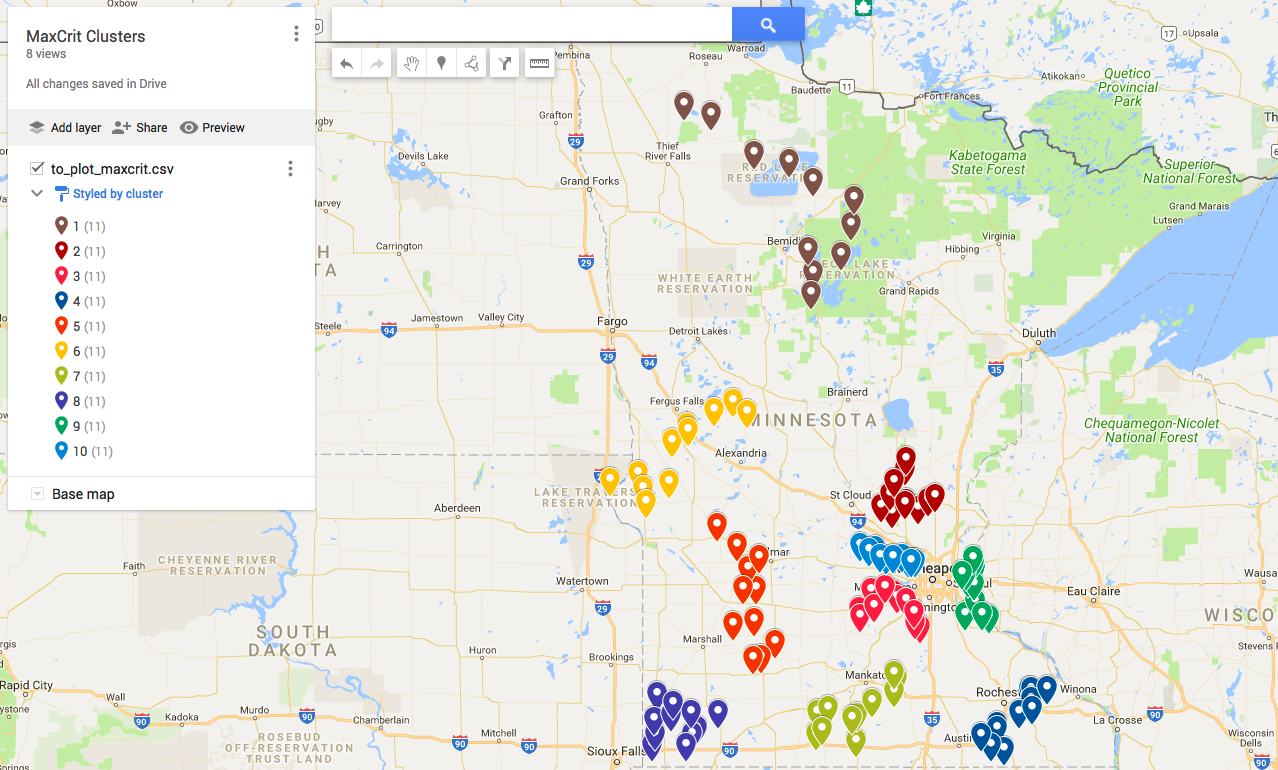
\includegraphics[width=.45\textwidth]{img/maxcrit_clusters.png}
\caption{Critical sets in Minnesota discovered using our methods. These are contiguous regions that lead to large measles outbreaks if not properly vaccinated.
\vspace*{-0.15in}
}
\label{fig:mn-criticalsets}
\end{figure}
%
%\begin{enumerate}
%\item 
\noindent
\textbf{1. Formalizing criticality.}
Building on the intuition from \cite{metcalf:epidemics15}, we formalize the notion of \emph{criticality} of a subset
$S\subseteq V$ in a social contact network $G=(V, E)$, as the \emph{expected number of additional infections} that would occur 
if the immunization rate within $S$ is ``low''  (e.g., compared to the state-wide rate). We estimate the criticalities of the clusters identified in \cite{cadena:vacc-cluster},
and observe that criticality is not correlated with the level of under-vaccination.
Extending this notion, we introduce the $\maxcrit{}$ problem: find a cluster $S$, which is
(1) contiguous in space, with respect to a spatial embedding network $\HR$ associated with $G$, 
and (2) has the maximum criticality.

The spatial proximity is motivated by the structure of clusters identified in 
\cite{lieu2015geographic,atwell:pediatrics13,cadena:vacc-cluster}, which are small and connected---this is desirable
from a public health response perspective, since interventions involve field work, which is most effective within a small region.

%We formalize the notion of criticality in a social contact network $G=(V, E)$, which is associated with a spatial embedding, represented as a graph $\HR$ (defined formally later). The criticality of a subset $S$ is defined as the \emph{expected number of additional infections} that would occur if the immunization rate within $S$ is low. We are interested in clusters $S$ that 1) are contiguous in space and 2) have the maximum criticality---this is referred to as the \maxcrit{} problem. The spatial proximity is motivated by a public health response perspective, as in \cite{lieu2015geographic,atwell:pediatrics13}. Public health interventions involve intensive field work, which is another motivation for clusters corresponding to contiguous regions. Further, such response is most effective within a small region. This motivates the problem of finding a contiguous spatial cluster $S$ of bounded size with maximum criticality. Our contributions are as follows.


\noindent
\textbf{2. Rigorous algorithms for $\maxcrit{}$.}
The $\maxcrit{}$ problem is computationally very challenging. We show that \maxcrit{} is NP-hard and design algorithm \algomaxcrit{}, which has a worst case approximation guarantee of $\Omega(1/k^{(d-1)/(2d-1)})$, relative to the optimum, for clusters of size $k$. Here, $d$ is the \emph{doubling dimension} of the graph (defined in Section \ref{sec:background}), and is related to the complexity of the spatial embedding network $\HR$, and it is a constant in practice---e.g., it is 2 for a grid graph.

\noindent
\textbf{3. Improved algorithms for submodular function maximization with connectivity.}
Our algorithm involves showing that the criticality function is submodular, which implies that $\maxcrit{}$ is a special case
of the problem of maximizing a non-negative monotone submodular function over the set of connected subgraphs of size $k$.
The best prior result for this problem is a $\Omega(1/\sqrt{k})$-approximation by Kuo et al~\cite{kuo2015maximizing}.
Since $1/k^{(d-1)/(2d-1)}\geq 1/\sqrt{k}$ for any $d\geq0$, \emph{our algorithm is the first improvement over the
result of \cite{kuo2015maximizing} for submodular maximization with connectivity constraints}.

We also show that $\maxcrit{}$ is equivalent to the classical problem of Influence Maximization (\infmax) \cite{kempe:sigkdd03},
\emph{with the the key difference that the seed set is connected}. This variant of \infmax{} has not been studied before,
and the only prior result is the $\Omega(1/\sqrt{k})$-approximation by applying \cite{kuo2015maximizing}.
Thus, our work also gives an improved result for the \infmax{} problem with connectivity constraint.


%Here, $d$ denotes the \emph{doubling dimension} of the associated spatial graph $\HR$ (defined later), and is a constant in practice, e.g., $2$ for a grid. We show that the \maxcrit{} objective is submodular, and this problem is equivalent to the classical Influence Maximization (\infmax) problem

%\item
\noindent
\textbf{4. Application.} 
We evaluate our algorithm on a detailed population and contact network model for the state of Minnesota.
The sets we discover have very high criticality compared to
heuristics commonly considered for public health interventions.
We achieve over 25\% higher criticality for the objective compared to all the baselines.
The critical clusters discovered using our algorithms (shown in Figure \ref{fig:mn-criticalsets})
have meaningful demographic properties
from a public health perspective: they typically involve people with lower than average
income and age (Section \ref{sec:experiments-cs}).
We also compute the criticalities of the clusters reported in \cite{cadena:vacc-cluster}.
Quite surprisingly, we find that: (1) the cluster with the lowest vaccination rate among these is not the most critical, and
(2) the cluster computed using our algorithm has criticality more than 10 times that of any of the clusters
identified by \cite{cadena:vacc-cluster}.

Finally, due to lack of publicly available high-resolution, geo-located outbreak data, there is no easy way to validate our results, but we note that \emph{one of the clusters we found to be critical lies in the Minneapolis metropolitan area where a large measles outbreak occurred in 2017 \cite{hall:mmwr17}}.

\noindent
\textbf{5. Social impact.}
Our method for finding critical sets, applied to detailed population and contact network models provides an operational tool for public health agencies in prioritizing their limited surveillance and public outreach resources towards the most critical clusters.
Our results imply that from a public health perspective, it is important to not only identify the undervaccinated clusters
as in~\cite{cadena:vacc-cluster}, but also determine which among them will likely cause an outbreak or an epidemic.






